\chapter{Evaluation}



explain the benchmarking setup and reason why certain setup choices were made

incorporate paper for statistical analysis which explains number of rounds etc

explain the benchmark problems and their specific attributes

show here that the approach in total is feasable

show the optimizations through better scheduling

discuss inexplicable results

\section{Local Distribution}

\begin{figure}[H]
	
	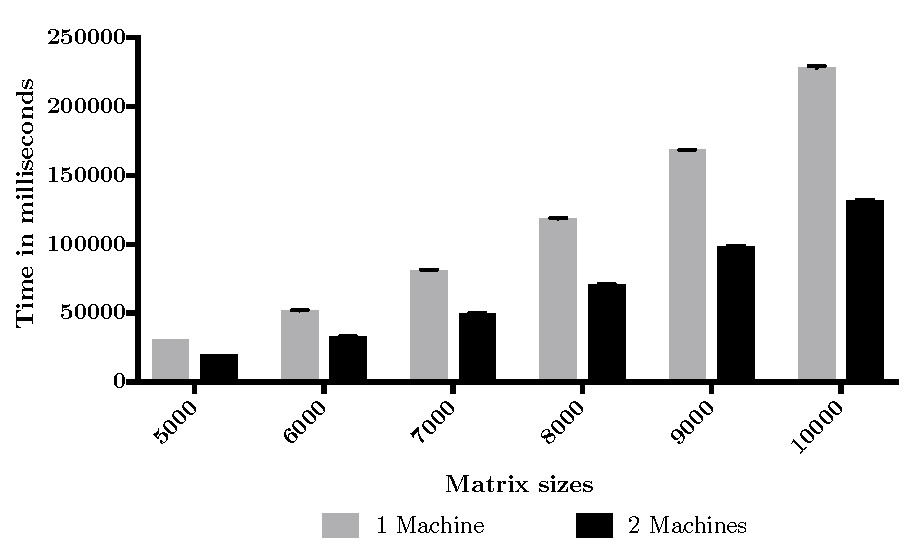
\includegraphics[width=1.0\textwidth]{images/sharded_matrix_multi.pdf}
	\centering
	\caption{Parallel Matrix Multiplication}
	\label{img:parallel_matrix}
\end{figure}


\begin{figure}[H]
	
	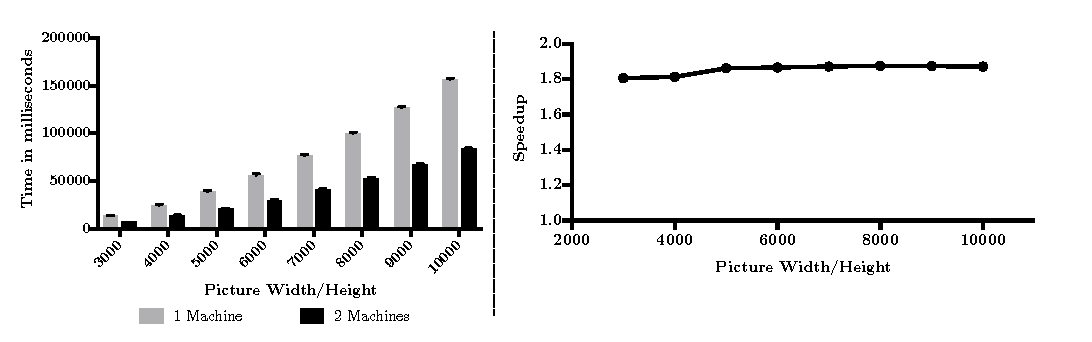
\includegraphics[width=1.0\textwidth]{images/sharded_mandelbrot.pdf}
	\centering
	\caption{Parallel Mandelbrot}
	\label{img:parallel_mandelbrot}
\end{figure}


\section{Hybrid Distribution}



benchmark selection
scheduler selection
benchmark setup: first submit all jobs, then start execution at once
why do iterative tasks have less kernels